
%En primer lugar para describir el diseño de la aplicación se describirán los requisitos del sistema
%necesarios para la ejecución de la aplicación, posteriormente comentaremos que herramientas se va usar a lo largo
%del desarrollo.

\paragraph{}
Al igual que en el apartado referente al análisis del sistema, en el diseño de este también usaremos una metodología orientada
a objetos mediante UML.

\paragraph{}
Este proceso es mucho más sencillo una vez que ya se ha especificado que hace el sistema en el capítulo anterior. También decir, que
al igual que el análisis del sistema, el diseño no contempla muchos detalles del sistema final, sólo una idea orientativa de como
se implementará el sistema.

\paragraph{}
En este capítulo no se han añadido descripciones de las clases que componen el sistema, para ello se encuentra disponible toda la
documentación del código, donde esta toda la información necesaria referente a las clases y archivos que componen la aplicación.

\section{Interfaz gráfica}

\paragraph{}
Tras los resultado que se han obtenido en la fase de análisis del sistema, es
necesario desarrollar una interfaz sencilla y agradable
para el usuario de la misma. En el diseño de estos, se intentará en todo momento que el usuario no tenga la posibilidad de insertar
datos erróneos que lleven a una ejecución anómala de la aplicación.

\begin{figure}[H]
  \label{interfaz}
  \begin{center}
    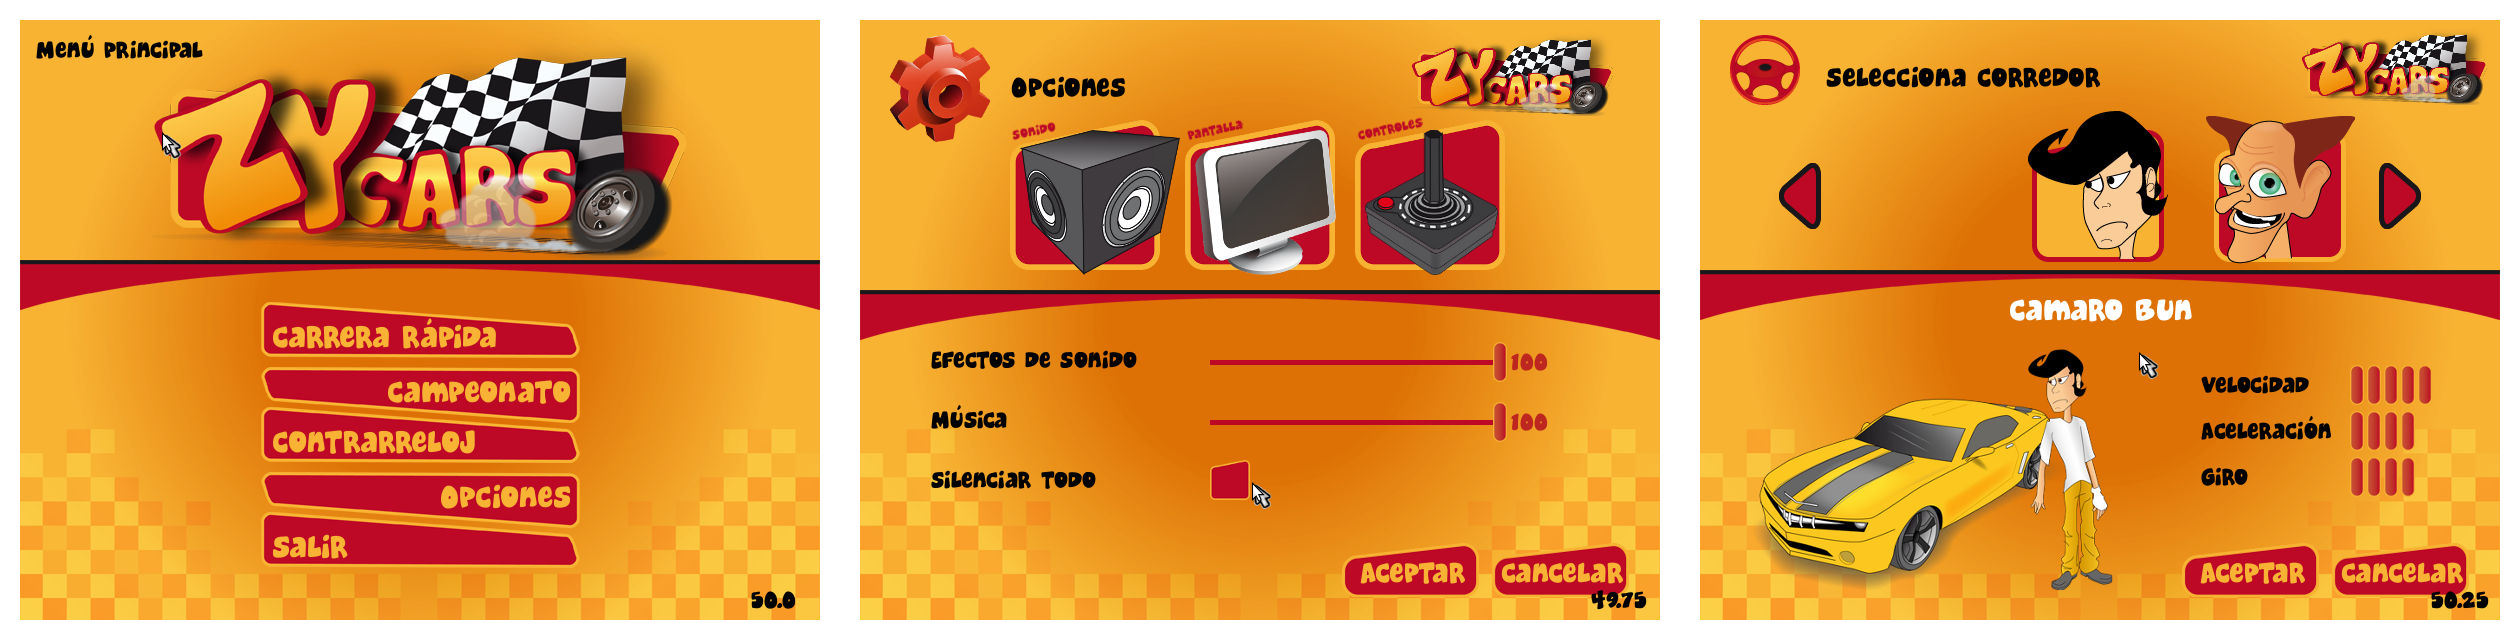
\includegraphics[scale=0.18]{imagenes/capturas/interfaz.png}
  \end{center}
  \caption{Diseño: Capturas de la interfaz del sistema}
\end{figure}

\subsection{Diagrama de interacción entre interfaces}

\paragraph{}
En la imagen que se muestra a continuación podemos observar la interacción
entre las distintas interfaces gráficas que se han 
desarrollado para la aplicación.

\begin{figure}[H]
  \label{diagrama_interaccion}
  \begin{center}
    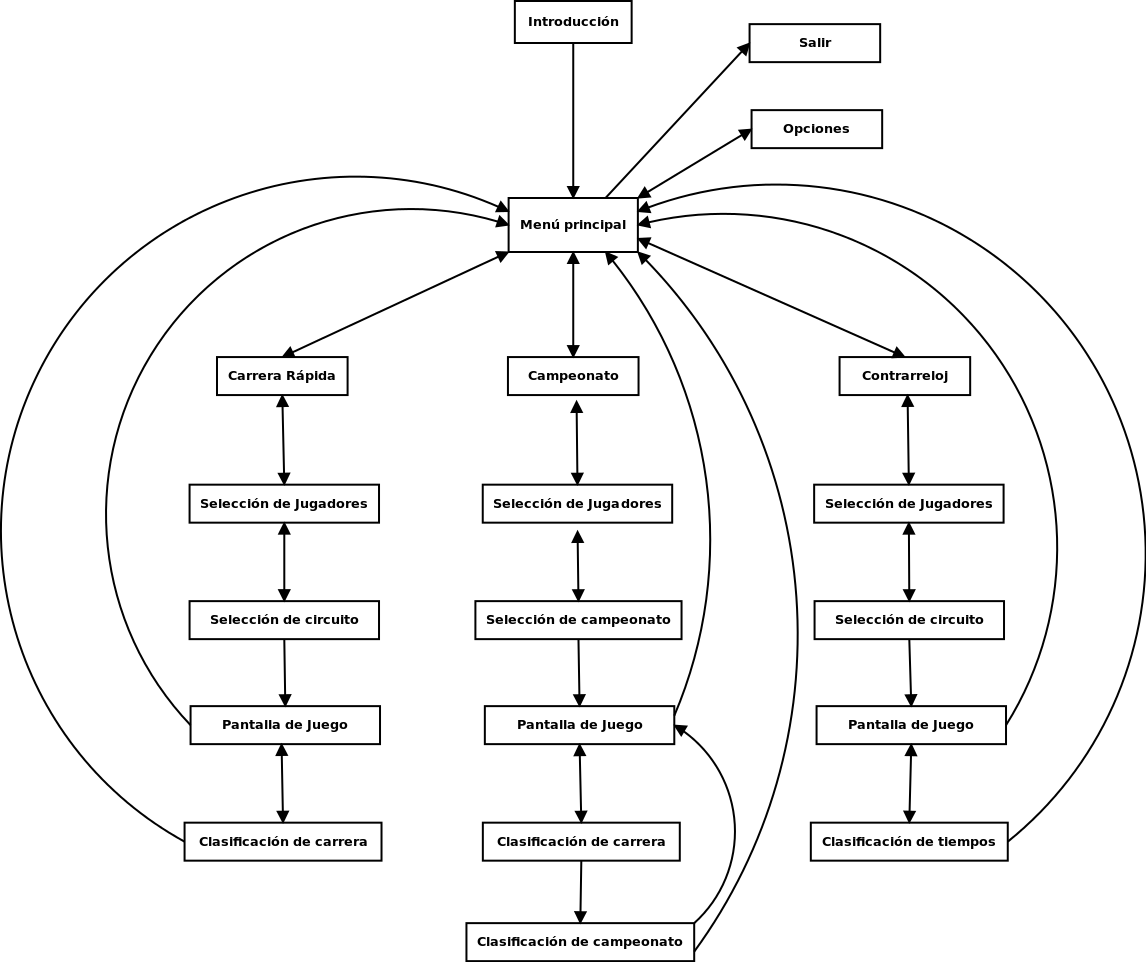
\includegraphics[scale=0.4]{imagenes/diseno/diagrama_interaccion.png}
  \end{center}
  \caption{Diseño: Diagrama de interacción}
\end{figure}

\section{Diagrama de clases de diseño}

\paragraph{}
Dividiremos el diagrama de clases de diseño en dos partes, para verlo con una mayor claridad, dicha separación se basará en el 
cometido de las clases que interfieran.

\paragraph{}
En primer lugar mostraremos todas las clases, encargada de inicializar el juego, y la gestión de los distintos estados que
podemos encontrar en este. Como pueden ser todos los menús en los que podremos interactuar en el sistema, mostrando la jerarquía 
de los mismos. Y también la clases encargadas de gestionar los tres modos de juego existentes, carrera rápida, contrarreloj y 
campeonato.

%\newpage

\begin{figure}[H]
  \label{diagrama_clases_diseno}
  \begin{center}
    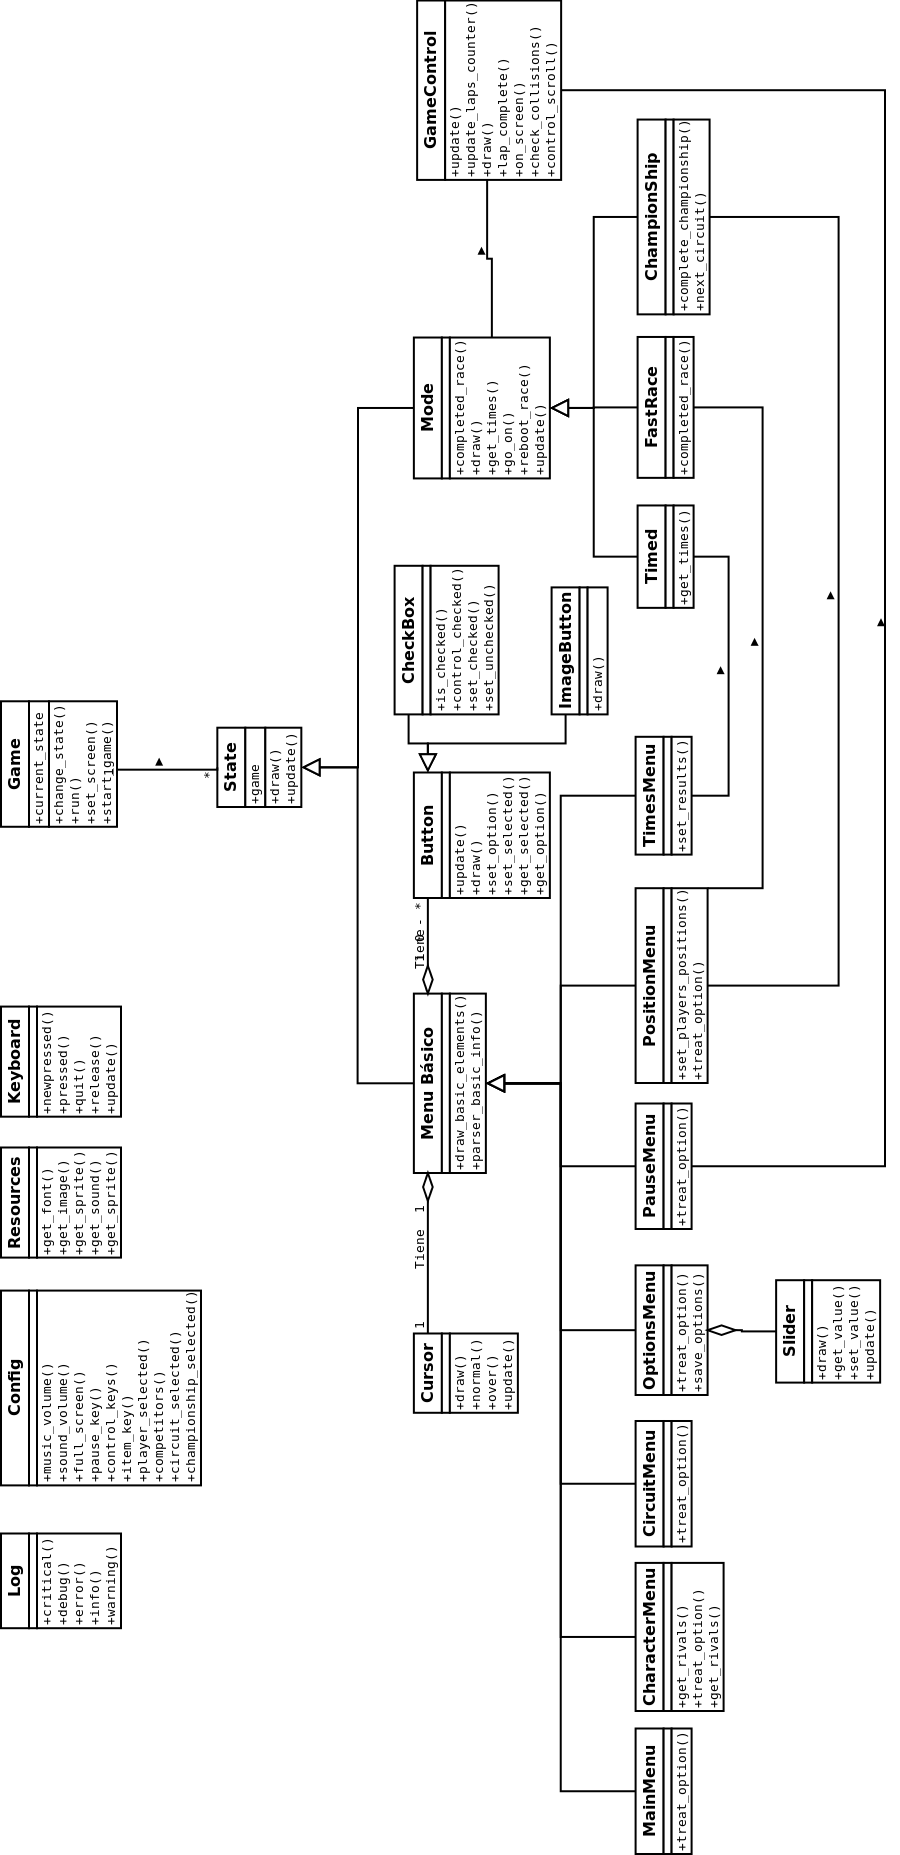
\includegraphics[scale=0.38]{imagenes/diseno/diagrama_clases_diseno1.png}
  \end{center}
  \caption{Diseño: Diagrama de clases de diseño 1}
\end{figure}

\paragraph{}
En el segundo diagrama mostraremos todas las clases relacionas con el sistema de juego. Podremos observar los distintos objetos que
intervienen en el juego, así como la jerarquía de estos. Y también todas las clases necesarias para el correcto funcionamiento del
juego.

\begin{figure}[H]
  \label{diagrama_clases_diseno}
  \begin{center}
    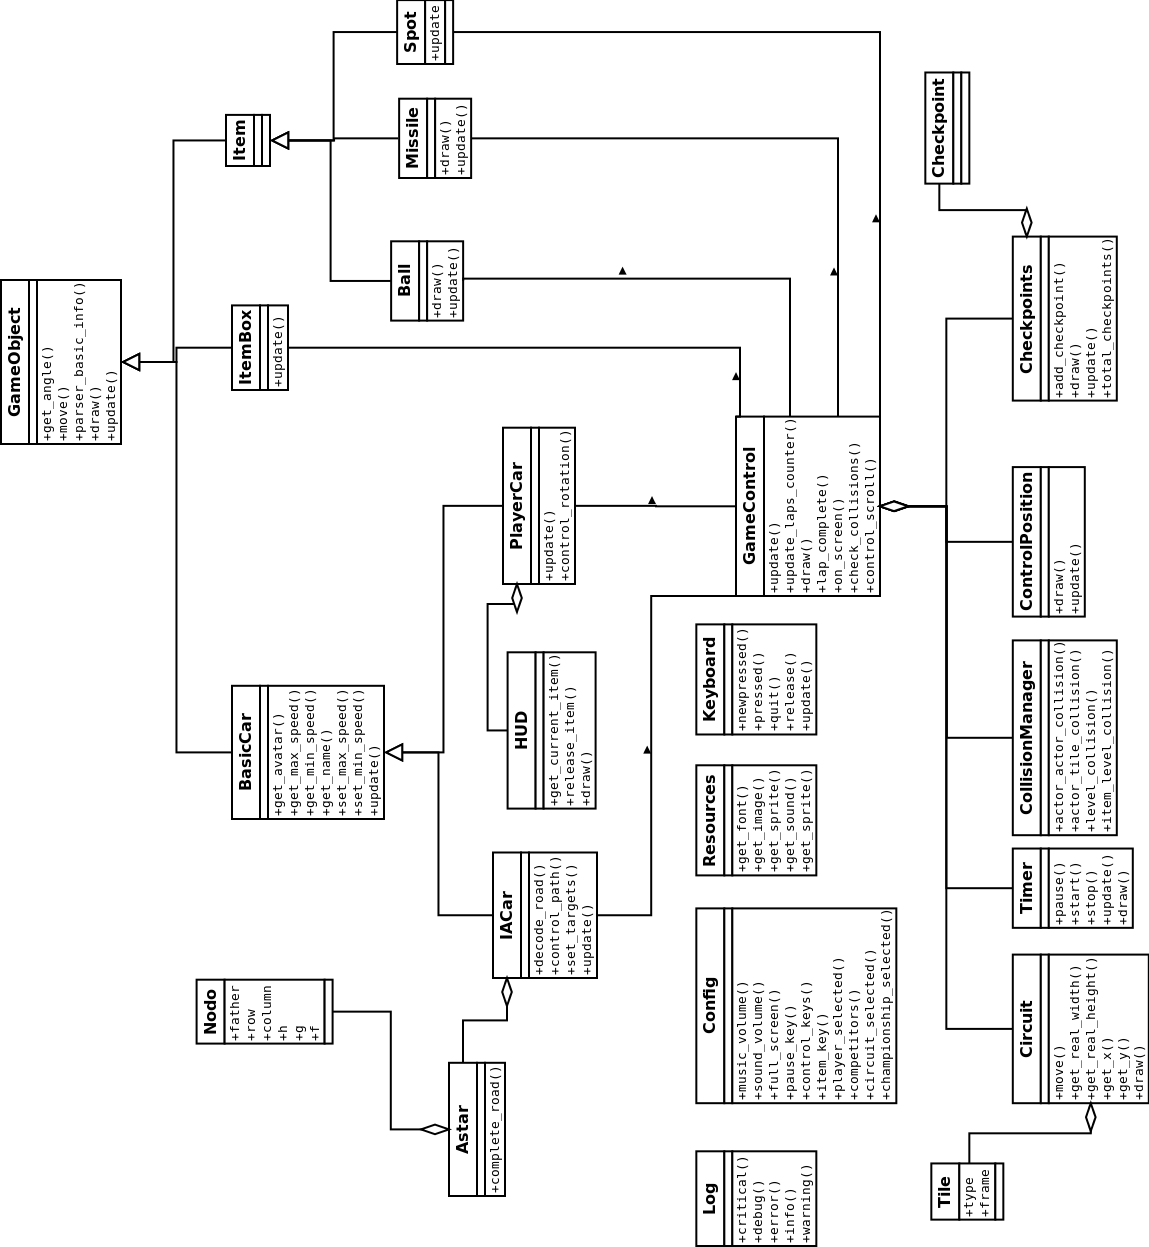
\includegraphics[scale=0.45]{imagenes/diseno/diagrama_clases_diseno2.png}
  \end{center}
  \caption{Diseño: Diagrama de clases de diseño 2}
\end{figure}

\section{Diagramas de secuencia}
lalalal
